\section{Benchmarks}\label{sec:benchmark}

In this section, we compare performances of 
various libraries against FastAD for a range of examples\footnotemark.
\footnotetext{github page: https://github.com/JamesYang007/ADBenchmark}
The following is an alphabetical list of the libraries used for benchmarking:\@
\begin{itemize}
    \item \href{http://www.met.reading.ac.uk/clouds/adept/}{Adept 2.0.8}
    \item \href{https://github.com/coin-or/ADOL-C}{ADOL-C 2.7.2}
    \item \href{https://coin-or.github.io/CppAD/doc/cppad.htm}{CppAD 20200000}
    \item \href{https://github.com/JamesYang007/FastAD}{FastAD 3.1.0}
    \item \href{https://github.com/trilinos/Trilinos/tree/master/packages/sacado}{Sacado 13.0.0}
    \item \href{https://github.com/stan-dev/math}{Stan Math Library 3.3.0}
\end{itemize}
All of the libraries are at their most recent release.
These libraries have also been used by others for 
benchmarking~\cite{carpenter:2015}\cite{margossian:2018}\cite{hogan:2014}.

The benchmark configuration is as follows:
\begin{itemize}
    \item \textbf{OS}: MacOSX Catalina Version 10.15.6 
    \item \textbf{Architecture}: x86 64-bit
    \item \textbf{Processor}: 3.4 GHz Quad-Core Intel Core i5
    \item \textbf{Compiler}: GCC10
    \item \textbf{C++ Standard}: 17
    \item \textbf{Compiler Flags}: 
\begin{verbatim}
    -O3 -march=native 
    -DNDEBUG 
    -DEIGEN_NO_DEBUG 
    -DADEPT_STACK_THREAD_UNSAFE 
    -D_REENTRANT 
    -DEIGEN_MATRIXBASE_PLUGIN="stan/math/prim/eigen_plugins.h" 
    -DEIGEN_ARRAYBASE_PLUGIN="stan/math/prim/eigen_plugins.h"
\end{verbatim}
    \item \textbf{FastAD Dependency}: \code{Eigen3.3.7}
\end{itemize}
While we used the newest GCC compiler, there is nothing in FastAD that relies on GCC10 specifically.
FastAD, however, requires the C++17 standard.
The \code{-O3} indicates maximum level of compiler optimization,
and \code{-march=native} exposes all of the available instruction sets 
such that the compiler can choose the best one.
The preprocessor definitions are to disable debugging
for best performance for all libraries, and some definitions were required by the libraries in order to compile.
Finally, FastAD has a dependency on \code{Eigen} matrix library,
but this is also a dependency for Stan.
The only application running was \code{iTerm2} (terminal),
the benchmark program, and system-related applications.

Compile time was not rigorously benchmarked, 
although we do note that adding code for Stan
increased compile time dramatically, which was also observed in~\cite{carpenter:2015}.
This is likely because Stan has numerous large dependencies such as Boost, Eigen, Sundial, and TBB.\@

All benchmarks benchmark the case where a user wishes to differentiate
a scalar function $f$ for different values of $x$.
This is a very common use-case.
For example, in the Newton-Raphson method,
we have to compute $f'(x_n)$ at every iteration with the updated $x_n$ value.
In HMC and NUTS, the leapfrog algorithm frequently
updates a quantity called the ``momentum vector'' $\rho$ 
with $\nabla_\theta \log(p(\theta, x))$ ($x$ here is treated as a constant),
where $\theta$ is a ``position vector'' that also gets frequently updated.

Our benchmark drivers are very similar to the one presented by Carpenter~\cite{carpenter:2015}.
In fact, we mainly took the same benchmark drivers, abstracted some details, and added a few more tests.
Every function to differentiate is defined as a functor and receives a single input,
which is a vector-like object of AD variables representing $x$.
For example, the \code{sum} functor is as follows:
\begin{lstlisting}[style=customcpp]
struct SumFunc
{
    template <class T>
    T operator()(const Eigen::Matrix<T, Eigen::Dynamic, 1>& x) const
    { return x.sum(); }

    adept::aReal operator()(const adept::aVector& x) const
    { return adept::sum(x); }

    auto operator()(const Eigen::Matrix<stan::math::var, Eigen::Dynamic, 1>& x) const
    { return stan::math::sum(x); }

    template <class T>
    auto operator()(ad::VarView<T, ad::vec>& x) const
    { return ad::sum(x); }

    void derivative(const Eigen::VectorXd& x,
                    Eigen::VectorXd& grad) const
    { grad = Eigen::VectorXd::Ones(x.size()); }

    std::string name() const { return "sum"; }

    void fill(Eigen::VectorXd& x) {
        for (int i = 0; i < x.size(); ++i) {
            x(i) = i;
        }
    }
};
\end{lstlisting}
All functors overload \code{operator()} to take in library-specific vector of AD variables.
Adept2.0 supports their own array feature and encourages the use of \code{aVector}.
FastAD supports the AD variable to have a vector-like shape by specifying the second template parameter as \code{ad::vec}.
All other libraries support a direct interface with~\code{Eigen::Matrix<AD variable type>}.
Some libraries provide built-in functions to evaluate the functor, and so we specialize whenever that is the case
to call these functions instead of performing the default (first) overload.
The default overload will always try to use \code{Eigen} API instead of manually written for-loops, as shown above.
However, if a function cannot be easily written with \code{Eigen} API, then a manually written code is used.
Every benchmark times the default overload for a vector of \code{double}s,
which will compute only the forward-evaluation, and this will serve as a baseline for all benchmarks.
This baseline will be denoted as \code{double} in the figures.
This approach was also used in~\cite{carpenter:2015},
however in our benchmark, the baseline is optimized to be vectorized,
whereas the reference uses a manual for-loop that may not be.
Hence, our results for all libraries with respect to the baseline may differ from those of the reference.
\code{name} returns an \code{std::string} object with a short name of the functor
and \code{fill} fills the initial values prior to starting any benchmarks. 

For brevity, the following is only a snippet of our main
benchmark function~\code{time\_gradients} that benchmarks Adept:
\begin{lstlisting}[style=customcpp]
    auto& adept_pack = packs.at(adb::TestName::adept);
    if (adept_pack.run) {
        adept::aVector x_ad(x.size());
        sw.start();
        for (int i = 0; i < adept_pack.n_iter; ++i) {
            adept_gradient(f, x, x_ad, fx, grad_fx);
        }
        sw.stop();
        check_gradient(grad_fx, expected, adept_pack.name);
        adept_pack.time = sw.elapsed() / adept_pack.n_iter;
    }
\end{lstlisting}
Other libraries are benchmarked in a similar way with \code{adept} replaced with the other library names.
\code{packs} is an \code{std::unordered\_map} mapping \code{TestName} enum value to a \code{TestPack} object
which contains information such as name of library, number of iterations to run, whether to run or not, etc.
This abstraction was only done to ease the programming and has no bearing on the actual benchmark results.
The first line grabs the \code{TestPack} object associated with Adept and checks if it should be run.
If so, it allocates a vector of AD variables.
The object \code{sw} is previously declared (not shown) as \code{StopWatch<>} and it is used as a stopwatch.
\code{StopWatch<>} is our own class that wraps \code{std::chrono::steady\_clock} to measure interval time.
The member function \code{start()} saves the starting time point and \code{end()} saves the ending time point.
Member function \code{elapsed()} returns the time elapsed in seconds between \code{begin()} and \code{end()} calls.
The elapsed time is computed in nanoseconds and then scaled by $10^{-9}$ to convert into seconds.
We measure the time it takes to differentiate \code{f}, \code{adept\_pack.n\_iter} times,
with the input \code{x} and the AD variable \code{x\_ad},
store the function result into \code{fx}, and save the gradient in \code{grad\_fx}.
For all benchmark examples, \code{n\_iter} is actually the same for all libraries and is set to 10000,
but for matrix multiplication, it is set to 1000 
since the complexity of the function was large enough to reach stable results with fewer iterations.
\code{f} is the functor representing the function to differentiate,
which was previously described in detail.
The function \code{check\_gradient} is for our debugging purposes to check accuracy.
Note that it is only called after the stopwatch finishes, so it does not affect the benchmark results.
All libraries had some numerical issues for some of the examples,
but the maximum proportion of error to the actual gradient values was on the order of $ 10^{-15}$, which is negligible.
Hence, in terms of accuracy, all libraries were equally acceptable.
Finally, we save the average time into \code{adept\_pack.time}.

Because FastAD works very differently from all of these libraries,
the benchmark setup is quite different:
\begin{lstlisting}[style=customcpp]
    auto& fastad_pack = packs.at(adb::TestName::fastad);
    if (fastad_pack.run) {
        Eigen::VectorXd val_buf;
        Eigen::VectorXd adj_buf;
        ad::VarView<double, ad::vec> x_ad(x.data(),
                                          grad_fx.data(),
                                          x.size());
        auto expr = f(x_ad);
        auto size_pack = expr.bind_cache_size();
        val_buf.resize(size_pack(0));
        adj_buf.resize(size_pack(1));
        expr.bind_cache({val_buf.data(), adj_buf.data()});
        sw.start();
        for (int i = 0; i < fastad_pack.n_iter; ++i) {
            fastad_gradient(expr, fx, grad_fx);
        }
        sw.stop();
        check_gradient(grad_fx, expected, fastad_pack.name);
        fastad_pack.time = sw.elapsed() / fastad_pack.n_iter;
    }
\end{lstlisting}
Section~\ref{ssec:example} already discussed the above code in detail.

We defined a gradient-computing function such as \code{adept\_gradient} for every library except for Stan,
since they already provided their own.
The code is exactly the same as the one used by Carpenter~\cite{carpenter:2015},
except that the allocations for the AD variables have been moved to before starting the stopwatch as shown above for Adept.
So, we do not show the code for these functions and 
direct the reader to the reference and the github page.
As for FastAD, the gradient function is extremely simple:
\begin{lstlisting}[style=customcpp]
    template <class ExprType>
    inline void fastad_gradient(ExprType& expr,
                                double& fx,
                                Eigen::VectorXd& grad_fx) 
    {
        grad_fx.setZero();
        fx = ad::autodiff(expr);
    }
\end{lstlisting}
It first sets the gradient to zero, which is required if multiple AD computations 
are carried out for the same expression viewing that gradient region.
Then \verb|ad::autodiff| both forward and backward-evaluates \verb|expr|
and stores the function value to \verb|fx|.
The backward-evaluation will update \verb|grad_fx| with the gradient values.

The main driver shown below is called \verb|run_test|, which calls
\verb|time_gradients| with various input sizes $N$.
\begin{lstlisting}[style=customcpp]
template <class F>
inline void run_test(F f, 
                     std::unordered_map<adb::TestName, adb::TestPack>& packs,
                     size_t max = 16 * 1024) 
{
    adept::Stack stack;
    std::string file_name = f.name() + "_eval.csv";
    std::fstream fs(file_name, std::fstream::out);
    print_results_header(fs, packs);
    for (int N = 1; N <= max; N *= 2) {
        std::cout << "N=" << N << std::endl;
        Eigen::VectorXd x(N);
        f.fill(x);
        time_gradients(f, x, packs, fs);
    }
}
\end{lstlisting}
The input vector size $N$ grows exponentially in powers of $ 2$ starting from $ 1$ to
$2^{14}$, and for each $N$ we fill the input vector \verb|x| using the functor and call \verb|time_gradients|.
This range of $N$ was enough to determine the asymptotic trend.

To the best of our abilities, we chose the most optimal code for each library 
that would be best suited for this particular scenario.
For example, Adept requires the user to define a stack object that saves the 
expression graph as well as the temporary values and adjoints for each node.
However, this stack object can be reused over many iterations.
Since a real use-case of Adept would likely reuse this stack object, we made this optimization.

For simplicity, we do not actually provide new $x$ values, but the benchmark code
is written as if $x$ may be different at every iteration; that is,
no optimizations were made for any libraries to exploit the fact that 
the $x$ values are actually kept the same.
This is important because most of the libraries require an initial step of creating AD variables
and copying the input values into the AD variables.
While we make the optimization to allocate these variables only one time for every library before the benchmark begins,
we cannot optimize-out the initialization
at every iteration to save the cost of copying.

The first few subsections will cover some micro-benchmarks where we benchmark commonly used functions: 
summation and product of elements in a vector, 
log-sum-exponential, 
matrix multiplication, 
and normal log-probability density function (pdf).
The last two subsections will cover some macro-benchmarks where we benchmark real-world examples: 
a regression model and a stochastic volatility model.

\subsection{Sum and Product}\label{ssec:sum_prod}

\begin{figure*}[t]
    \centering
    \begin{subfigure}[b]{0.475\textwidth}
        \centering
        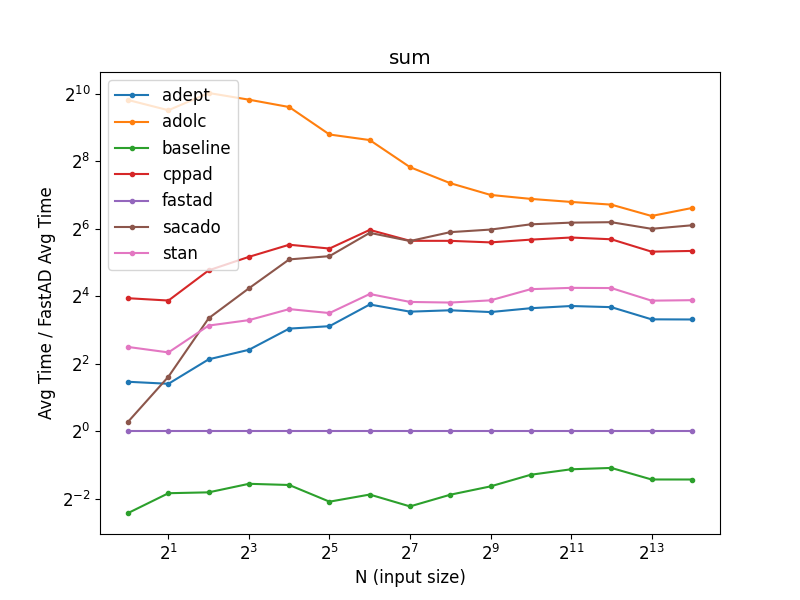
\includegraphics[width=\textwidth]{figs/sum_fig.png}
        \caption{Sum}\label{fig:sum}
    \end{subfigure}
    \hfill
    \begin{subfigure}[b]{0.475\textwidth}
        \centering
        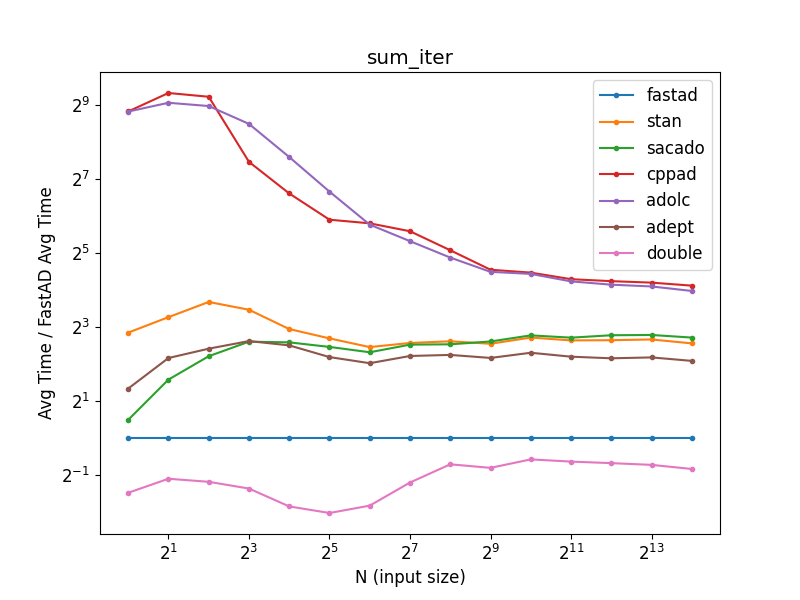
\includegraphics[width=\textwidth]{figs/sum_iter_fig.png}
        \caption{Sum (naive, for-loop-based)}\label{fig:sum_iter}
    \end{subfigure}
    \vskip\baselineskip%
    \begin{subfigure}[b]{0.475\textwidth}
        \centering
        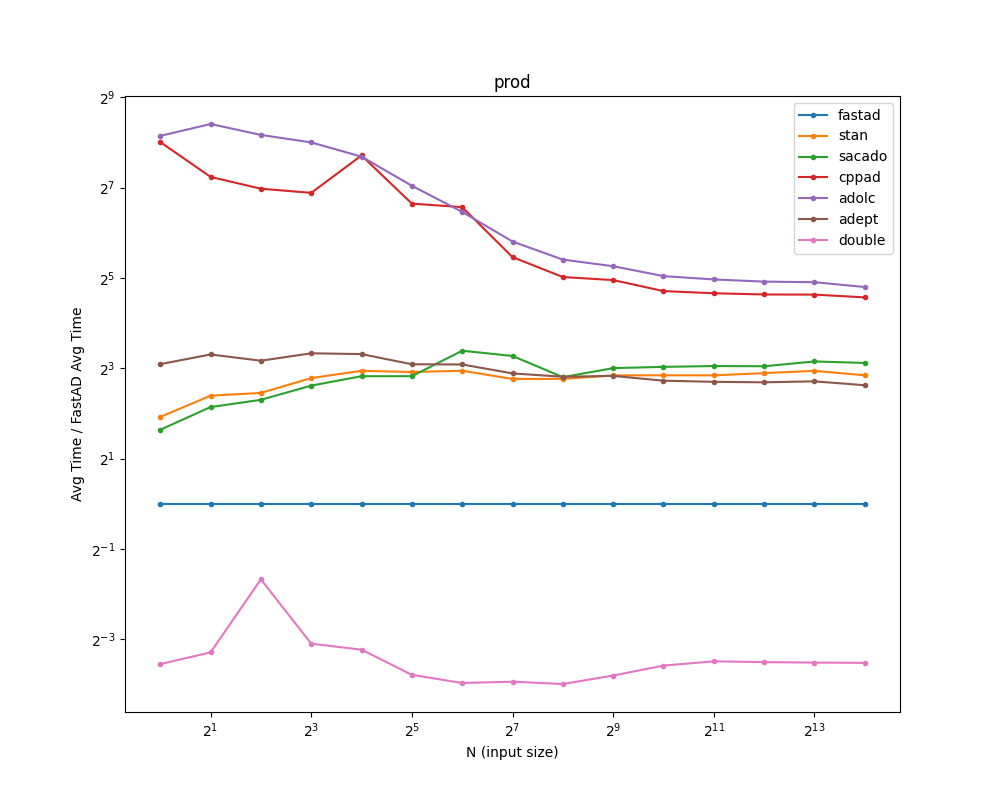
\includegraphics[width=\textwidth]{figs/prod_fig.png}
        \caption{Product}\label{fig:prod}
    \end{subfigure}
    \hfill
    \begin{subfigure}[b]{0.475\textwidth}
        \centering
        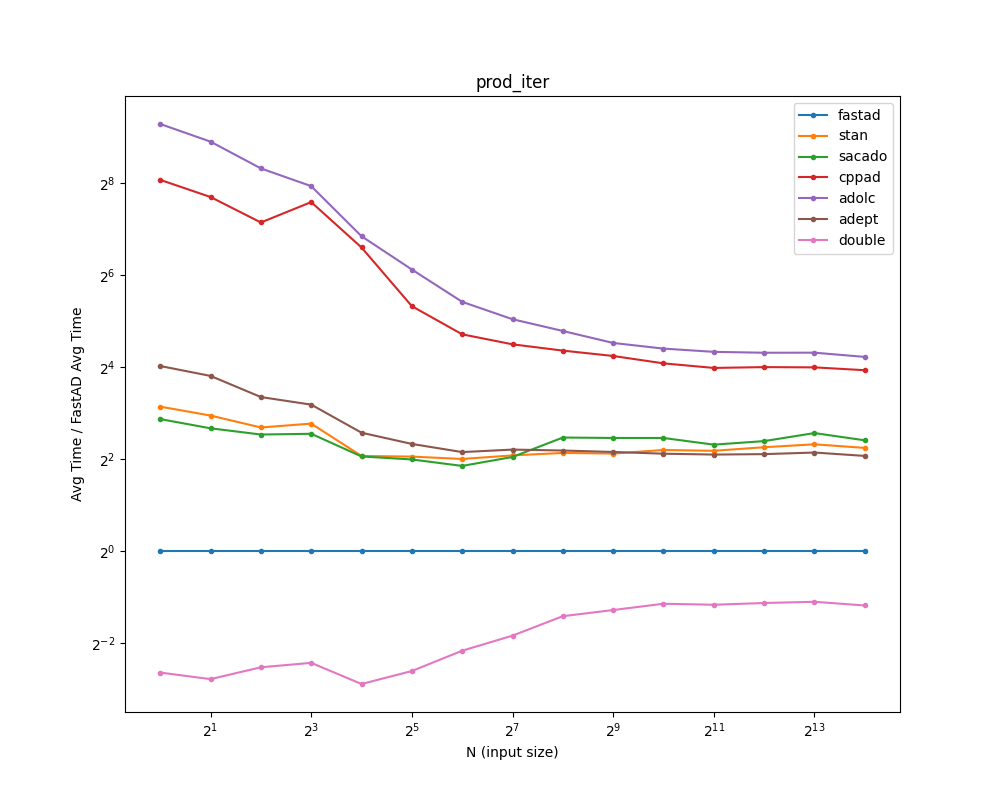
\includegraphics[width=\textwidth]{figs/prod_iter_fig.png}
        \caption{Product (naive, for-loop-based)}\label{fig:prod_iter}
    \end{subfigure}
    \caption{%
        Sum and product benchmarks of other libraries against FastAD 
        plotted relative to FastAD average time.
        Fig.~\ref{fig:sum},\ref{fig:prod} use built-in functions whenever available.
        Fig.~\ref{fig:sum_iter},\ref{fig:prod_iter} use the naive iterative-based code for all libraries.
    }\label{fig:sum_prod}
\end{figure*}

The summation function is defined as $f_s:\R^n \to \R$ where~$f_s(x) = \sum\limits_{i=1}^n x_i$,
and the product function is defined as $f_p:\R^n \to \R$ where~$f_p(x) = \prod\limits_{i=1}^n x_i$.
The only libraries supporting a built-in function for summation are Adept, FastAD, and Stan;
those that support product are Adept and FastAD.\@
All other libraries use the \verb|Eigen| API:
\begin{lstlisting}[style=customcpp]
    template <class T>
    T operator()(const Eigen::Matrix<T, Eigen::Dynamic, 1>& x) const
    { return x.sum(); }
\end{lstlisting}
As another test, we forced all libraries to use the manually-written for-loop-based summation and product.
Fig.\ref{fig:sum_prod} shows the benchmark results.

In all four cases, it is clear that FastAD outperforms all libraries for all values of $N$
by a significant factor.
For \verb|sum|, Fig.\ref{fig:sum} shows that, asymptotically, 
the next three fastest libraries are Adept, Stan, and Sacado, respectively.
The trend stabilizes starting from $N=2^6=64$ where Adept is about $ 12$ times slower than
FastAD, Stan about $ 18$ times, and Sacado about $ 74$ times.
The naive, for-loop-based benchmark shown in Fig.\ref{fig:sum_iter} exhibits a similar pattern,
although the performance difference with FastAD is less extreme:
Adept is about $ 4$ times slower, 
Stan about $ 6$ times,
and Sacado about $ 6.5$ times.
Nonetheless, this is still a very notable difference.
Although the difference between FastAD and the \verb|double| baseline is much larger in
the \verb|sum| case (2.56 times slower than baseline) than 
\verb|sum_iter| (1.76 times slower than baseline), 
this does not mean that \verb|sum| was slower.
In fact, in terms of absolute time, \verb|sum| was $ 5$ times faster than \verb|sum_iter|. 
Rather this means that the backward-evaluation in the case for \verb|sum| was
as expensive as the forward-evaluation, but in the case for \verb|sum_iter|,
backward-evaluation was much cheaper relative to the forward-evaluation.
This makes sense because \verb|sum| is vectorized and hence takes much shorter time to evaluate
than \verb|sum_iter|, and in both cases the backward-evaluation simply sets the partial derivatives to $ 1$.

For the \verb|prod| and \verb|prod_iter| cases, 
Fig.\ref{fig:prod},\ref{fig:prod_iter} again show
a similar trend as \verb|sum| and \verb|sum_iter|.
Overall, the comparison with FastAD is less extreme.
For \verb|prod|, Adept is about $ 5.6$ times slower than FastAD,
Stan about $ 7.3$ times slower,
and Sacado about $ 16.4$ times slower.
For \verb|prod_iter|, Adept is about $2.9$ times slower,
Stan about $4$ times slower,
and Sacado about $4.6$ times slower.


\subsection{Log-Sum-Exp}

\begin{figure*}[t]
    \centering
    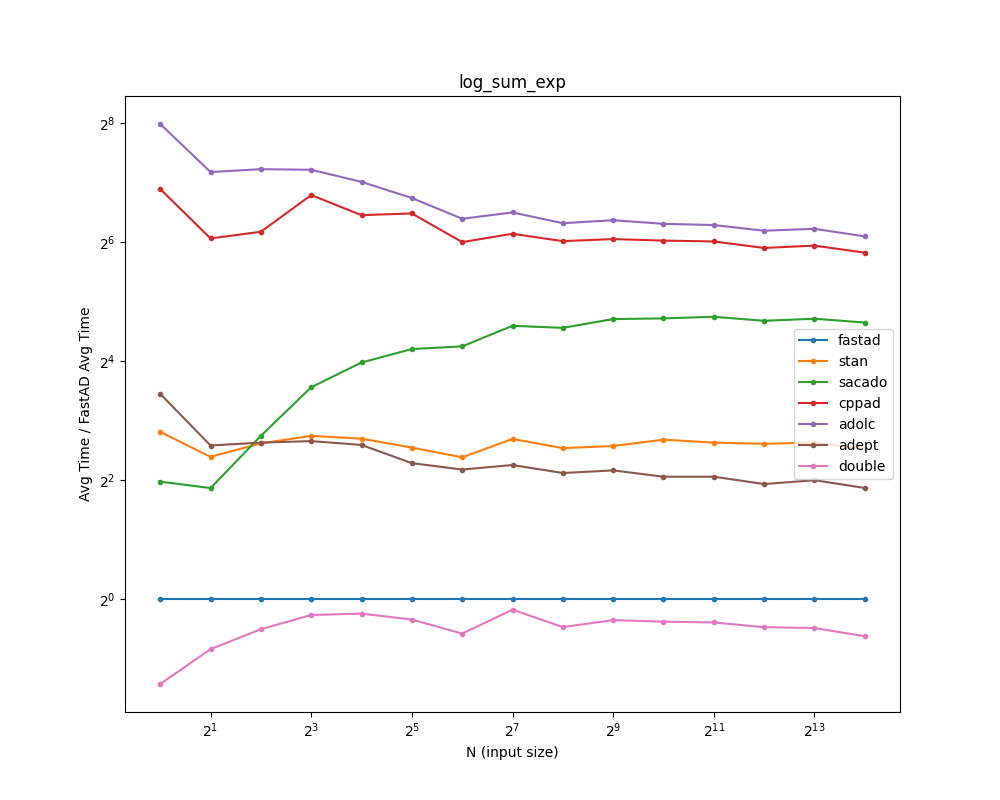
\includegraphics[width=0.8\textwidth]{figs/log_sum_exp_fig.png}
    \caption{%
        Log-sum-exp benchmark of other libraries against FastAD 
        plotted relative to FastAD average time.
    }\label{fig:log_sum_exp}
\end{figure*}

The log-sum-exp function is defined as $f:\R^n \to \R$ 
where~$f(x) = \log(\sum\limits_{i=1}^n e^{x_i})$,
Fig.~\ref{fig:log_sum_exp} shows the benchmark results.

FastAD outperforms all libraries for all values of $N$.
The next three fastest libraries are Adept, Stan, and CppAD, respectively.
The trend stabilizes starting from $N=2^6=64$ where 
Adept is about $ 2.5$ times slower than FastAD, 
and Stan about $ 7.7$ times.
Note that FastAD is only marginally slower than the baseline,
especially for small to moderate values of $N$,
despite calls to expensive functions like \code{log} and \code{exp}.
In fact, at the largest value of $N = 2^{14}$, 
FastAD is $ 1.5$ times slower than the baseline, 
meaning there is about $ 50\%$
overhead from one forward-evaluation to also compute the gradient.
This is because FastAD is optimized such that in this case
the forward-evaluated result for \code{exp} expression is reused
during the backward-evaluation.


\subsection{Matrix Multiplication}\label{ssec:matrix_mult}

\begin{figure*}[t]
    \centering
    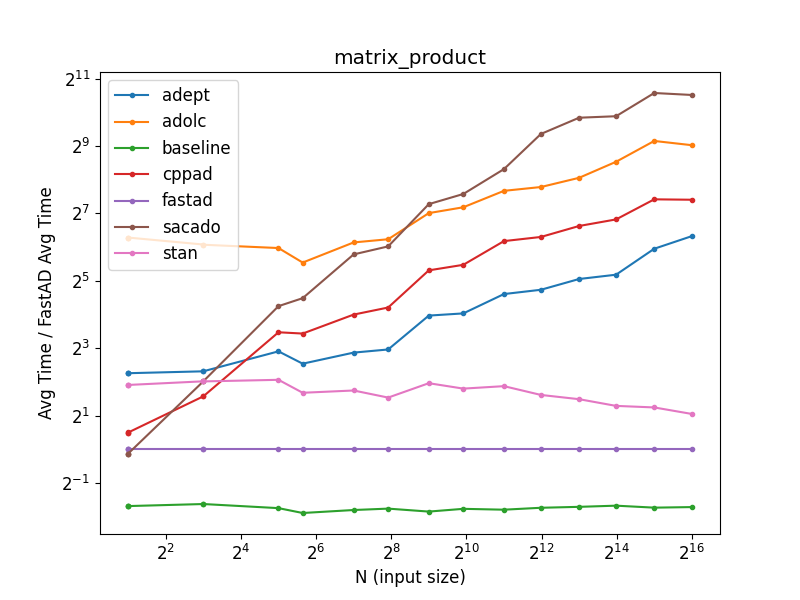
\includegraphics[width=\textwidth]{figs/matrix_product_fig.png}
    \caption{%
        Matrix multiplication benchmark of other libraries against FastAD 
        plotted relative to FastAD average time.
    }\label{fig:matrix_mult}
\end{figure*}

For this benchmark, all matrices are square matrices of the same size.
The functor fills the x vector by first resizing it to $2 \cdot K^2$,
where each matrix is $K\times K$.
In order to have a scalar target function,
we add another step of adding all of the entries of the matrix multiplication, i.e.
\[
    f(A, B) = \sum\limits_{i=1}^{K} \sum\limits_{j=1}^{K} {(A \cdot B)}_{ij}
\]
Hence, we could not benchmark with $N$ at exact powers of $ 2$,
however, the modified range of values for $N$ still shows a meaningful trend.
We also tested $N$ larger than $2^{14}$ since it was not enough to show any convergent behavior.
All libraries except Adept and Stan were excluded from this benchmark
because they did not provide suitable support for matrix multiplication
and the default overload using \verb|Eigen| API exceeded the time limit.
All tested libraries provide built-in functions to 
compute the matrix multiplication and sum the elements.
Fig.\ref{fig:matrix_mult} shows the benchmark results.

FastAD is still the fastest library for all values of $N$, 
but Stan performs much closer to FastAD than in the previous examples.
Adept consistently performs worse compared to FastAD and Stan.
The trend stabilizes towards the end at around $N=2^{14}$ where 
Stan is about $ 2$ times slower.
For moderate sized $N \in [2^{8}, 2^{10}]$, Stan is about 3--4 times slower.

The comparison with the baseline shows that FastAD takes $ 3.14$ times longer.
Note that forward-evaluation requires one matrix multiplication between two $N\times N$ matrices,
and backward-evaluation additionally requires two matrix multiplications of the same order,
one for each adjoint:
\begin{align*}
    \frac{\partial f}{\partial A} 
    &= \frac{\partial f}{\partial (A\cdot B)} \cdot B^T \\
    \frac{\partial f}{\partial B} 
    &= A^T \cdot \frac{\partial f}{\partial (A\cdot B)}
\end{align*}
Hence, in total, one AD evaluation requires three matrix multiplications between two $N\times N$ matrices.
As a rough estimate, if we approximate a manually-written gradient computation to be
three times the baseline (one multiplication), FastAD time relative to this approximate manual gradient computation time
is $\frac{3.14}{3} = 1.0475$.
This shows then that FastAD only has about $ 4.75\%$ overhead 
from a manually-written code, which is extremely optimal.


\subsection{Normal Log-PDF}\label{ssec:normal_log_pdf}

\begin{figure*}[t]
    \centering
    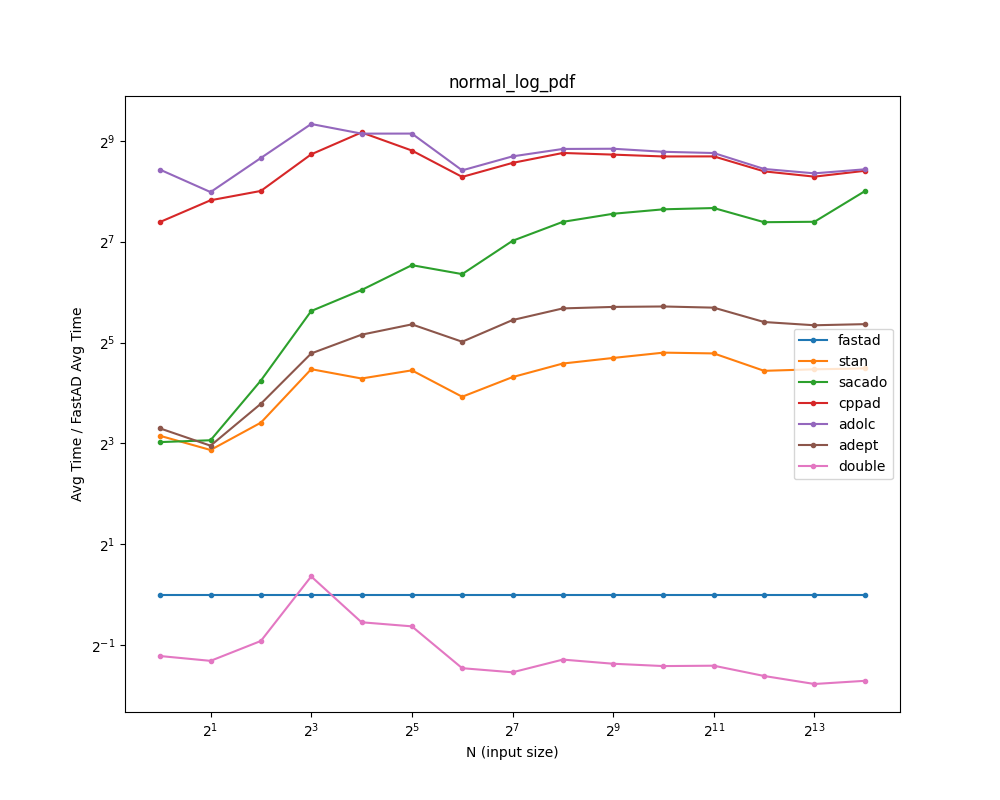
\includegraphics[width=0.7\textwidth]{figs/normal_log_pdf_fig.png}
    \caption{%
        Normal log-pdf benchmark of other libraries against FastAD 
        plotted relative to FastAD average time.
    }\label{fig:normal_log_pdf}
\end{figure*}

The normal log-pdf function is defined up to a constant as:
\[
    f(x) = -\frac{1}{2\sigma^2} \sum\limits_{i=1}^N \paren{x_i - \mu}^2 
           -N\log(\sigma)
\]
For this benchmark, $\mu = -0.56,\,\sigma = 1.37$ and are kept as constants.
Fig.~\ref{fig:normal_log_pdf} shows the benchmark results.

FastAD is the fastest library for all values of $N$.
The trend stabilizes at around $N=2^{7}=128$.
Towards the end, Adept is about $ 9$ times slower,
and Stan about $ 19$ times slower.
Comparing all libraries,
the overall difference we see in this example is the largest we have seen so far,
and this is partly due to how we compute $\log(\sigma)$.
Section~\ref{ssec:compile-time-opt} showed that we can check at compile-time
whether a certain variable is a constant, in which case,
we can perform a more optimized routine.
In this case, since $\sigma$ is a constant, it computes the normalizing constant
$\log(\sigma)$ once and gets reused over multiple AD evaluations 
with no additional cost during runtime,
which saves a lot of time since logarithm is a relatively expensive function.


\subsection{Bayesian Linear Regression}\label{ssec:regression}

\begin{figure*}[t]
    \centering
    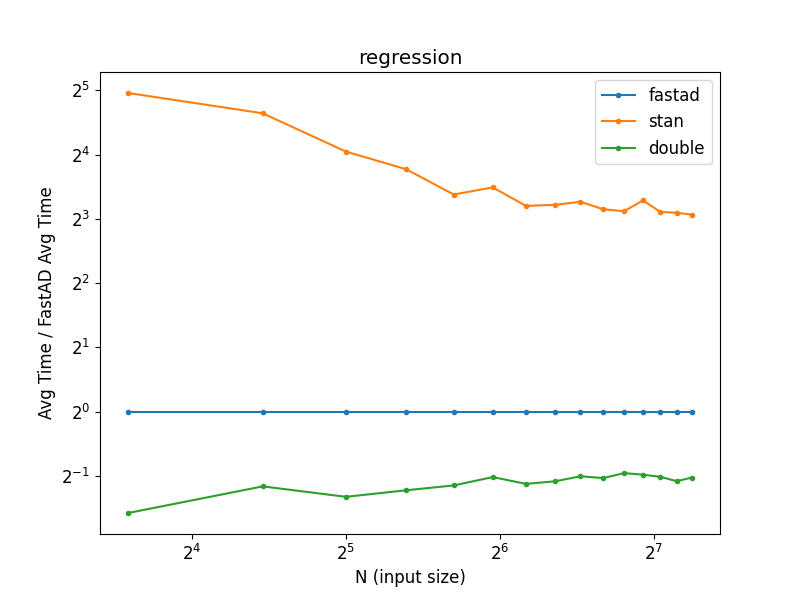
\includegraphics[width=0.75\textwidth]{figs/regression_fig.png}
    \caption{%
        Bayesian linear regression benchmark of Stan against FastAD 
        plotted relative to FastAD average time.
    }\label{fig:regression}
\end{figure*}

This section marks the first macro-benchmark example.
We consider the following Bayesian linear regression model:
\begin{align*}
    y &\sim N\paren{X\cdot w + b, \sigma^2} \\
    w &\sim N\paren{0,1} \\
    b &\sim N\paren{0,1} \\
    \sigma &\sim Unif\paren{0.1, 10.}
\end{align*}
The target function is the log of the joint probability density function (up to a constant).
Fig.~\ref{fig:regression} shows the benchmark results.

FastAD outperforms Stan by $ 8.6$ times for the largest $N$ and Adept by $ 10$ times.
The trend stabilizes starting from around $N=70$.
It is interesting to see that around $N=2^7$, 
FastAD is only $ 2.2$ times slower than the baseline,
despite the model consisting of a large matrix multiplication and many normal log-pdfs.
One of the reasons is that the compiler was able to optimize-out the backward-evaluation 
of the matrix constant $X$, since constants implement a no-op for backward-evaluation.

If we assume that the most expensive operation is the matrix multiplication,
AD evaluation approximately takes two matrix multiplications between a matrix and a vector.
We can then approximate a lower bound for the manually-written gradient computation time to be two times that of the baseline.
The relative time of FastAD to this approximated time is
$1.1$, implying about $ 10\%$ overhead from a manually-written code.


\subsection{Stochastic Volatility}\label{ssec:stochastic_volatility}

\begin{figure*}[t]
    \centering
    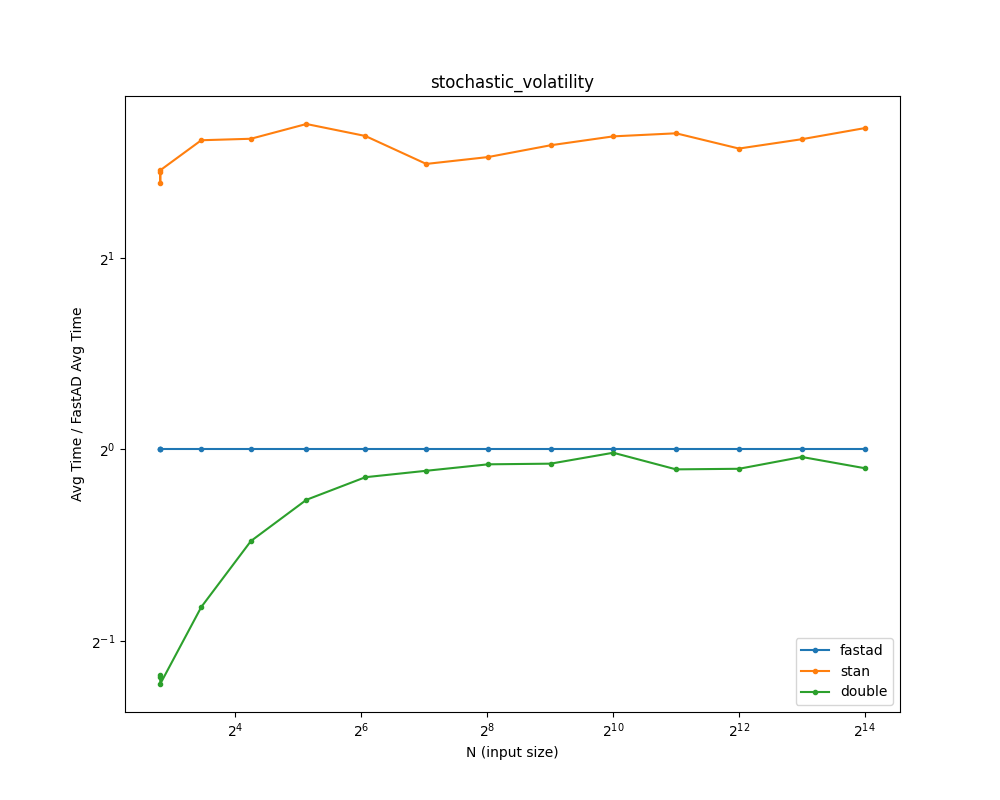
\includegraphics[width=0.8\textwidth]{figs/stochastic_volatility_fig.png}
    \caption{%
        Stochastic volatility benchmark of Stan against FastAD 
        plotted relative to FastAD average time.
    }\label{fig:stochastic_volatility}
\end{figure*}

This section marks the second and last macro-benchmark example.
We consider the following stochastic volatility model 
taken from the Stan user guide~\cite{stan-rm:2018}:
\begin{align*}
    y &\sim N(0, e^{h}) \\
    h_{std} &\sim N(0, 1) \\
    \sigma &\sim Cauchy(0,5) \\
    \mu &\sim Cauchy(0,10) \\
    \phi &\sim Unif(-1, 1) \\
    h &= h_{std} \cdot \sigma \\
    h[0] &= \frac{h[0]}{\sqrt{1 - \phi^2}} \\
    h &= h + \mu \\
    h[i] &= \phi \cdot (h[i-1] - \mu),\, i > 0
\end{align*}
The target function is the log of the joint probability density function (up to a constant)
and we wish to differentiate it with respect to $h_{std}, h, \phi, \sigma, \mu$.
For this benchmark, we only consider Stan for the same reasons described in Section~\ref{ssec:regression}.
The fill function for this functor will resize a vector of size $N$ as $\tilde{N} = N + 3$,
where the first $N/2$ values refer to $h_{std}$,
the next $N/2$ values refer to $h$,
and the next three refer to $\phi, \sigma, \mu$, respectively.
We take care of the edge case where $N < 2$ to let $N = 2$ and then carry out the steps above.
Here, $y$ is a constant.
All quantities are randomly generated uniformly in $(-1,1)$ range
and $\sigma$ is modified afterwards to be strictly positive.
Fig.\ref{fig:stochastic_volatility} shows the benchmark results.

FastAD outperforms Stan by 3 times for the largest $N$.
The trend seems quite stabilized from the start.
It is interesting to see that FastAD is only marginally slower than the \code{double} baseline
for moderate to large $N$ values.
The ratio between FastAD time to baseline time is $ 1.07$, which means there is about a $7\%$ overhead 
just from one \emph{forward-evaluation} to \emph{also} compute the gradient.
Hence, gradient computation is almost free from just computing the log-pdf,
which puts FastAD at near-optimal performance.

